\documentclass{article}
\usepackage{comment}
\usepackage[final]{styles}
\usepackage[utf8]{inputenc} % allow utf-8 input
\usepackage[T1]{fontenc}    % use 8-bit T1 fonts
\PassOptionsToPackage{hyphens}{url}\usepackage{hyperref}       % hyperlinks
\usepackage{url}            % simple URL typesetting
\usepackage{booktabs}       % professional-quality tables
\usepackage{amsfonts}       % blackboard math symbols
\usepackage{nicefrac}       % compact symbols for 1/2, etc.
\usepackage{microtype}      % microtypography
\usepackage{amsmath}
\usepackage{amsthm}
\usepackage{amssymb}
\usepackage{tikz}
\usepackage{csquotes}
\usepackage{float}
\usepackage{graphicx}
\usepackage{wrapfig}
\usepackage{multicol}

% \title{Harmonic Flows on Guage Equivariant Moduli Space of Connection }
% \title{Ergodic Flows on Guage Equivariant \\ Space of Connection }
% \title{Ergodic flow on Moduli\\  Space of Connections }
% \title{Attention and Energy Minimization \\ on Moduli  Space of Connections }
\title{Energy Minimizing Flows on \\ Equivariant Space of Connections }
% \title{Learning Energy Minimization on \\  Moduli Space of Connections }

% The \author macro works with any number of authors. There are two commands
% used to separate the names and addresses of multiple authors: \And and \AND.
%
% Using \And between authors leaves it to LaTeX to determine where to break the
% lines. Using \AND forces a line break at that point. So, if LaTeX puts 3 of 4
% authors names on the first line, and the last on the second line, try using
% \AND instead of \And before the third author name.

\author{%
  L. J. Pereira \\
%   \texttt{lukejoepereira@gmail.com} \\
  % examples of more authors
  % \And
  % Coauthor \\
  % Affiliation \\ consciousness
  % Address \\
  % \texttt{email} \\
  % \AND
  % Coauthor \\
  % Affiliation \\
  % Address \\
  % \texttt{email} \\
  % \And
  % Coauthor \\
  % Affiliation \\
  % Address \\
  % \texttt{email} \\
  % \And
  % Coauthor \\
  % Affiliation \\
  % Address \\
  % \texttt{email} \\
}

\begin{document}
\setlength{\abovedisplayskip}{4pt}
\setlength{\belowdisplayskip}{4pt}

\vspace{-2cm}
\maketitle


\vspace{-1.3cm}

\begin{comment}
\begin{abstract}

% A novel energy-based learning model is described using gauge theory and is speculated to produce dynamics similar to those in found in neuronal activity. 
In gauge theory, the moduli space of connections results from quotienting the space of principal connections of a fiber or vector bundle by the structure group, generating a gauge equivariant space. A moduli space of connections can be used to cover the activity of a collection of deep neural networks, which are represented as trajectories on vector bundles. On this upper bounding space, a top-down energy-based attention mechanism can be trained from activity of the bottom-up trajectories of the underlying networks through a composition of energies. Dynamics of attention are computed by minimizing the energy functional of the space; in particular, the Yang-Mills moduli space, a subset of the total connection space, can be constructed to be a smooth, compact, and oriented manifold in 4 dimensions with critical points known as Yang-Mills connections (or instantons). 
% The harmonic model can be applied to these dynamics with behaviour comparable to connectome-specific self-localized critical waves. 
Examining mathematical research in ergodic and hyperbolic dynamics of moduli spaces allows the ergodic free-energy minimizing model described in previous works to be developed further.
An autoencoding method using the cobordism property of the space is considered.

% This yang mills space of connection curvature can be represented with holomorphic vector bundles on which variational noise generates energy-based attention. In a statistical learning and information geometry setting, this space can be viewed as a kernel manifold which interfaces with specialist neural networks in a product of experts summation. This formulation of general intelligence provides a simple and biologically plausible model of 
 

% Fiber bundles of manifolds from differential geometry can be applied to the meta-learning task of the classification of subtasks to subnetworks. Assuming the input of a typical machine learning task can be associated with some Lie Group, then a differentiable manfiold can be constructed to represent the space of all tasks. Using gauge theory, this manifold can be  formalized as a Yang-mills moduli space.
\end{abstract}

\end{comment}

% gauge Dynamics of moduli spaces
\section{Overview}
In gauge theory, the moduli space of connections results from quotienting the space of principal connections of a fiber or vector bundle by the structure group, generating a gauge equivariant parameter space. A moduli space of connections can be used to cover the activity of a collection of hierarchical or deep neural networks, represented as trajectories on vector bundles. On this upper bounding space, a top-down energy-based attention mechanism, referred to as the moduli attention, can be trained from sampled activity of the bottom-up trajectories of underlying networks through a composition of energies. Dynamics of attention are computed by minimizing the energy functional of the connection space. In particular, the Yang-Mills moduli space, a subset of the total connection space, can be constructed to be a smooth, compact, and oriented manifold in 4 dimensions with critical points known as Yang-Mills connections (or instantons). These connections minimize curvature between bundles and, from an information geometric perspective, they minimize relative entropy or KL divergence between gauge equivariant manifolds. Allowing these connections to function as sources of variational noise, we train a neural network to minimize total energy of the moduli space. This process can be understood as finding stable solutions of an intrinsic flow on the curvature metric, producing a Ricci Yang-Mills flow with solutions akin to Ricci solitons. Stable solutions represent islands of agreement formed through consensus within a dynamic part-whole hierarchy. The theoretical objects representing solutions of these flows are studied as quasiparticles and can be made physical in quantum materials or gasses. This geometric formulation of general intelligence is a naturally arising and biologically plausible model for quantum AI. 
% Moreover, fusing physical field theories with neuroscience and ML may justify introspection into the Anthropic Principle and cosmological fine-tuning. 

% Exploratory musings in quantum machine learning describe a quasiparticle in a bose-enstein condesate of the Yang-mills moduli space described earlier. To do so, a control system must train the condesate using boltzman machines to allow the quasiparticle to endure. This quasiparticle represents the state of the Moduli space of connections  after a Wick rotation of the 4-dimensional space into bosons in 3-dimensional space.
% by minimizing the relative entropy or KL divergence between active bundles.
% The harmonic model can be applied to these dynamics with behaviour comparable to connectome-specific self-localized critical waves. 


\section{Geometry of Latent Information}
\subsection{Manifolds, Vector bundles, Connections}
    A fiber bundle serves as a useful mathematical object to analyse both the recursive construction of artificial and biological neurons and neural networks, as well as providing fitting descriptions of the geometry of latent information, which uses manifold representations for information processing and statistical learning.
    % Finer details can be found in my notebooks on differential geometry, Lie groups and algebras, and gauge theory.
    A fiber bundle formalizes the notion of one topological space (called a fiber) being parameterized by another topological space (called a base). The bundle is equipped with a group action on the fiber that represents different ways the fibers can be viewed as equivalent. Bundles also have a property, known as local trivialization, allowing neighborhoods of the bundle to be computed as simple, oriented product spaces, despite the global space  being unoriented or twisted.
    
    A family of fibers associated to a base can be described by defining a standard (or template) fiber which all other fibers are isomporphic to. This is formalized by defining a diffeomorphic or homotopic projection mapping, that connects positional data from the entirety of the space of fibers to a base, and implicitly from one fiber to another. When the template fiber is a vector space, the bundle is called a vector bundle. Similarly, a standard connections between fibers exists, known as a principal Ehresmann connection, and can be understood as a covariant directional derivative on the tangent spaces of the manifolds. Intuitively understood, Lie groups have a special recursive nature as a result of the group itself being a differentiable manifold of a continuous symmetry. A useful phenomenon occurs when equipping a bundle with a Lie group action; the bundle structure can be used to represent both the original vector bundle as well as a higher-level collection of mappings of their tangent spaces, in what's known as a bundle of connections. 
    % To be expanded in the section on moduli spaces, the Yang-Mills or instanton connections within this bundle of connections correspond to those that minimize their curvature. 
    
% \newpage
    

\subsection{A Priori Structure Groups}
    
    % Hebbian learning is a form of activity-dependent synaptic plasticity where correlated activation of pre- and postsynaptic neurons leads to the strengthening of the connection between the two neurons. Another central theory of cognitive neuroscience is that different parts or modules of the brain perform different functions, known as functional localization.
    % We can develop a simple partition scheme by initially assigning a Bernoulli random variable to each synapse. Then, while ``zooming out" we merge random variables together based on their covariance and locality to build a course-grained model. Recall, \textit{covariance} is a measure of the joint variability of two random variables and is increasingly positive when the variables tend to show similar behavior and grow increasingly negative when dissimilar. This conversion of physical synapses into a set of random variables can be described with Markov partitions and Bernoulli Schemes. 
    % At each step, the accuracy of the model naturally decrease as a result of merging imperfectly covariant random variables.
    %     However, some form of a priori covariance is necessary for maintaining information integrity through bilateral and hierarchical dynamics, i.e. to allow a connection to communicate in a general and equivariant way between modules and within their intrinsic substructures. 
    
    % \begin{wrapfigure}{r}{0.5\textwidth}
    %     \begin{center}
    %     \includegraphics[width=0.43\textwidth]{DTI-sagittal-fibers.jpg}
    %     % \caption{Fiber tracts that run through the mid-sagittal plane}
    %     \end{center}
    % \end{wrapfigure}
    
   A biological first principle of covariance arises naturally from analysis of neuronal activity, which favours functional localization and Hebbian learning.
    Moreover, cognitive networks in the brain flow in connectome-specific diffusive waves along gyrification paths, which are theorized to be caused by differential tangential growth. 
    Recall, covariance is a measure of the joint variability of a pair random variables and is increasingly positive when the pair show similar behavior and is negative when dissimilar.
    Moving from discrete random variables (i.e. synapses) to  and continuous fields and manifolds (i.e. EM fields), the covariant derivative between fibers of a bundle naturally arises and is known as a principal Ehressmann connection. To allow holonomy of dynamics on a bundle, it is necessary to impose a generalized a priori covariance principle to maintain integrity of information during parallel transportion in bilateral and hierarchical directions.
    Yet for a standard learning model, covariance of functionality is an a posteriori feature since the joint variability is unknown until individual modules are fully trained. 
    Covariance of fibers can be achieved by imposing the structure group to be a Lie Group, but can also be achieved by imposing restrictions on the projection map of Riemannian manifolds without explicitly defining the structure group beforehand (Gao 2021).
    
    % \begin{figure}[h]
    %     \centering
    %     \includegraphics[width=5.5cm]{DTI-sagittal-fibers.jpg}
    %     \caption{Fiber tracts that run through the mid-sagittal plane}
    % \end{figure}
    
    % \begin{figure}[h]
    %     \centering
    %     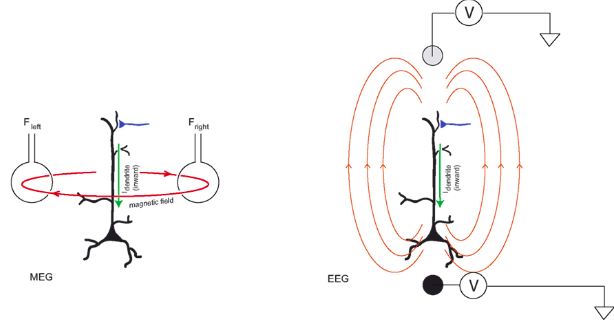
\includegraphics[width=8cm]{eeg-meg-neuron.png}
    %     \caption{Diffusive electric and magnetic signals in neurons}
    % \end{figure}

    
    
\subsection{Moduli Spaces}
    With covariance established on connections, it becomes possible to perform inference using higher levels of abstraction on gauge fields. This is done by constructing a gauge equivariant bundle of connections known as a moduli space of connections, which can be further reduced to a Yang-Mills moduli space defined to be a finite dimensional manifold. This reduced space has local and global minima being connections with minimized energy known as Yang-Mills connections or instantons. Yang-Mills connections serve as a natural choice of connection on principal and vector bundles since they minimize their curvature. From an information geometric perspective, this can be thought of as minimizing relative entropy between sampled trajectories of manifolds which happen to be gauge equivariant. This infinitesimal form of the the Kullback–Leibler divergence (or relative entropy) is comparable to the Fisher information metric. The gauge field strength is the curvature $F_{A}$ of the connection, and the energy of the gauge field is given by the Yang–Mills action functional:
    \begin{equation}
         {\displaystyle \operatorname {YM} (A)=\int _{X}\|F_{A}\|^{2}\,d\mathrm {vol} _{g}.}
    \end{equation}
    With the aim of having zero or vanishing curvature, we vary paramaters in search of a connection with curvature as small as possible. The Yang–Mills action functional simply corresponds to the $L^{2}$-norm of the curvature, and its Euler–Lagrange equations describe the critical points of this functional, either the absolute minima or local minima.   

% \vspace{-0.3cm}
\section{Variational Geometric Flows}
\subsection{Variational Inference and Energy Composition}
    As underlying neural networks perform inference, their latent trajectories pass through layers of a neural network in a bottom-up manner. At the same time, a top-down variational noise is produced around the instanton solutions that best minimize energy of the total activity on the moduli space of connections. Using an energy-based model (EBM) we sample the joint distribution as a sum of each latent trajectory, corresponding to a product of experts model. This forms an attention mechanism, which we refer to as the moduli attention, and is learned on the top-down manifold while having a generative effect on underlying networks through approximate inference. It has recently been implemented using Stein Variational Gradient Descent algorithm (Jaini 2021). Recall, variational methods pick a family of distributions over the latent variables with their own variational parameters, $q(z_{1:m} | v)$, then attempt to find settings of the parameters that makes $q$ close to the posterior of interest. Closeness of the two distributions is measured with the Kullback-Leibler (KL) divergence, 
    \begin{equation}
         \displaystyle KL(q||p)=  E_q\bigg[ \log \frac{ q(z)}{p(z | x)} \bigg].
    \end{equation}
    % $ \ \ \displaystyle KL(q||p)=  E_q\bigg[ \log \frac{ q(z)}{p(z | x)} \bigg].
    % $
    \begin{figure}[H]
        \centering
        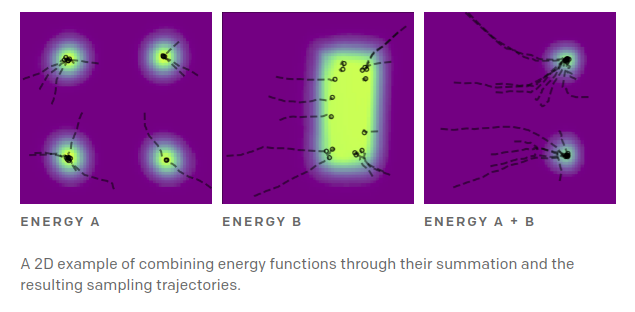
\includegraphics[width=13cm]{openai-ebm.png}
        \vspace{-0.87cm}
        \\  (Yilun, 2019)
        % \caption{Fiber tracts that run through the mid-sagittal plane}
    \end{figure}


\subsection{Geometric Flows}
    
    \begin{wrapfigure}{r}{0.4\textwidth}
        \vspace{0.3cm}
        \centering
        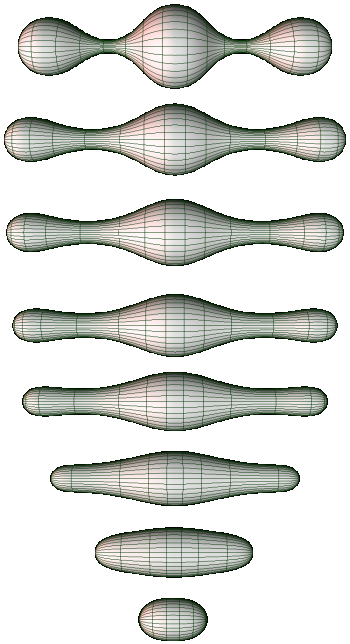
\includegraphics[scale=0.3]{ricci-flow.png}
        % \caption{Ricci flow visualization (Rubinstein, 2005)}
        \\ Ricci flow of a metric manifold (Rubinstein, 2005)
    \end{wrapfigure}
    
    We can interpret energy minimization as a geometric flow, either on the parameter space as an extrinsic flow through variational gradient descent, or on the moduli space as an intrinsic flow. A Ricci flow is an example of an intrinsic flow on the metric by which one can take an arbitrary manifold and smooth out the geometry to make it more symmetric, whereas a mean curvature flow (as found in soap films, with critical points as minimal surfaces) is an example of an extrinsic flow on an embedded manifold. The moduli attention mechanism can be understood as a mix of the two categories; manipulating both the embedded manifolds constructed from hierarchical neural networks and the moduli space of connections (or metric) itself. We can further classify it as both a variational and a curvature flow since it evolves to minimize the Yang-mills action functional which is the $L^2$ norm of curvatures. 
    % The Ricci flow, Calabi flow, and Yamabe flow all arise in similar ways. 
    Curvature flows may not necessarily preserve volume (the Calabi flow does, while the Ricci flow does not), meaning the flow may simply shrink or grow the manifold, rather than regularizing the metric. Instead of normalizing the flow by fixing the volume, we allow dissaptive solutions to exist, forming a memory and compression mechanism. 

\subsection{Islands in Part-Whole Hierarchies}
    The GLOM model (Hinton 2021) aims to represent part-whole hierarchies, using islands of matching vectors, known as islands of agreement, to construct nodes in parse tree representations within a neural network. A part-whole hierachy is a system consisting of components that can themselves be further broken down into subcomponents. The model learns intuition and analogical reasoning by finding clusters of coherence which encodes parts that are not well defined, unconscious, or possibly obscured. Moreover, Hinton describes the importance of viewpoint and coordinate-invariance allowing for exchangeability within the network, which can be used to adapt to and generate novelty, similar to creativity in humans. We can draw comparisons between the GLOM model and moduli attention, where vector encodings correspond to dynamic trajectories on vector bundles, frame invariance corresponds to the gauge equivariant space of connections, and islands of agreement correspond to using variational, curvature geometric flows that manifest semi-stable instanton or soliton solutions. 
    
    Iterative consensus generally does not converge in coherent ways because of the difficulty of encoding a prior understanding of desirable representations to be generated through agglomerative clustering. However, using a geometric model we find that we are better posed to converge to coherent clusters because of the use of an a priori structure group that imposes meaningful symmetry on the clusters and optimizes organization of information throughout the space. Moreover, using geometric flows to analyse the process, we gain access to a trove of mathematical research on the solubility, stability, and other convergence properties and behaviour.
    
\subsection{Variational Methods in EBMs}
    An energy function $E$ in an EBM can be thought of as an unnormalized negative log probability (LeCun 2020). 
    To convert an energy function to its equivalent probabilistic representation after normalization,
    % Recall, marginalisation is a method that sums over the possible values of one variable to determine the marginal contribution of another. 
    $P(y \mid x)$, we apply the Gibbs-Boltzmann formula with latent variables $z$ being marginalized implicitly through integration, i.e. $P(y \mid x) = \int_z P(y,z | x)$. Then,
    \begin{align*}
        P(y \mid x) &= \frac{ \int_z \exp(-\beta E(x,y,z)) }{ \int_y \int_z \exp(-\beta E(x, y, z))} 
    \end{align*}
    The derivation introduces a $\beta$ term which is the inverse of temperature $T$, so as $\beta \rightarrow \infty$ the temperature goes to zero, and we see that $\check{y} = \text{argmin}_{y} E(x,y)$. This inverse temperature limit appears similar to the critical temperature in a Bose-Einstein Condesate (BEC). We can redefine our energy function as an equivalent function with free energy $F_\beta$,
    \begin{align*}
        F_{\infty} (x,y) &= \text{argmin}_z E(x,y,z)\\
        F_{\beta} (x,y) &= -\frac{1}{\beta} \log \int_z \exp(-\beta E(x,y,z)).
    \end{align*}
    If we have a latent variable model and want to eliminate the latent variable $z$ in a probabilistically correct way, we just need to redefine the energy function in terms of $F_\beta$,
    \begin{equation}
         P(y \mid x) = \frac{ \exp(-\beta F_\beta(x,y,z)) }{ \int_y \exp(-\beta F_\beta(x, y, z))}.
    \end{equation}
    With variational methods, instead of only minimizing the energy function with respect to $z$ we must prevent the energy function from being 0 everywhere by constraining the flexibility of the latent variable $z$. The energy function is defined as sampling $z$ randomly according to a distribution whose logarithm is the cost that links it to $z$. This distribution is commonly chosen to be a Gaussian with mean $\bar z$ which results in Gaussian noise being added to $\bar z$. The reparameterization trick is often used to allow for backpropagation during training despite the random sampling.

    \section{Topological Quantum Computing (Exploratory)}

     % \subsection{Solitons and Instantons}
    \subsection{Quasiparticles}
    
    % \begin{comment}
    % quasiparticles and collective excitations
    % - Instantons and solitons
    
    % - Ricci solitons
    % https://math.stackexchange.com/questions/802933/ricci-soliton-geometric-meaning
    
    % - RICCI YANG-MILLS SOLITONS
    % https://arxiv.org/pdf/0907.1095.pdf
    % https://arxiv.org/pdf/2102.09538.pdf
    
    % \end{comment}
    
    Quasiparticles and collective excitations are emergent phenomena that encapsulate sections of a microscopically complicated system with their behaviour imitating different behaviour of weakly interacting particles in a vacuum. 
    A soliton is a localized, non-dispersive solution of a nonlinear theory in Euclidean space and is a real object. Conversely, instantons are not real and only exist as solutions to the equations of motion of a quantum field theory after a Wick rotation, in which time is made imaginary. Note, a Wick rotation is a transformation that substitutes an imaginary-number variable for a real-number variable in order to solve a problem of (complex) Minkowski space in Euclidean space. Therefore, instantons are not observable, but are used to calculate and explain quantum mechanical effects that can be observed, such as tunneling. In quantum chromodynamics (QCD), instantons are believed to tunnel between the topologically different color vacua.
    
    Aside from providing a computational schema, it's worth noting the philosophical implications of associating physical unified field theories with neuroscience and machine learning theory. Namely, that it  may justify further introspection into the Anthropic Principle and cosmological fine-tuning.

    \subsection{Ricci Yang-Mills solitons}
    
    A Ricci flow is a differential equation on the space of Riemannian metrics on $M, \mathfrak{Met}$. We can picture the Ricci flow as moving a manifold around by internal symmetries (the family of diffeomorphisms) and a uniform-in-space scaling at each time. If one works in the moduli space of $\mathfrak{Met}/ \mathfrak{Diff}$, where $\mathfrak{Diff}$ is the group of diffeomorphisms on $M$, then one allows for a family of fixed points that are metrics that flow by scaling and diffeomorphism. i.e. $g(t) = \sigma (t) \phi (t) ^* g_0$,
    where $\phi(t) :M \rightarrow M$ is a one parameter family of diffeomorphisms. 
    These are the Ricci soliton metrics. 
    In the standard quantum field theoretic interpretation of the Ricci flow in terms of the renormalization group, the parameter $t$ corresponds to length or energy rather than time.
    One can show that Ricci soliton metrics satisfy the following equation: $Rc+\mathcal{L}_X g+ 
    \frac{\epsilon}{2} g = 0$, where $X$ is the vector field generating the diffeomorphisms, and $\epsilon = -1,0,1$ corresponds to shrinking, steady,and expanding solitons, respectively. If $X$ is the gradient of some function, i.e.$X=\triangledown f$, then a solution is said to be a gradient Ricci soliton.
    
    The Ricci Yang-Mills flow is a natural coupling of the Ricci flow and the Yang-Mills heat flow. It was discovered that the Ricci Yang-Mills flow is an ideal candidate for studying magnetic flows. Given a choice $h$ of metric on the Lie algebra $g$ of $G$, a one-parameter family of metrics $g_t$ on $\Sigma$ and principal connections $\mu_t$ satisfies the Ricci-Yang-Mills flow (RYM flow) if, 
    \begin{equation}
        \frac{\partial}{\partial t} g = -2 Rc \ g + F^2_\mu,  \ \ \ \ \ \ \ \ \ \ \ \ \ 
        \frac{\partial}{\partial t}\mu = -d^*_gF_\mu .
    \end{equation}
    \subsection{Bose-Einstein Condesate}
    
    A Bose–Einstein condensate (BEC) is a state of matter which is typically formed when a gas of bosons at low densities is cooled to temperatures very close to absolute zero causing a large fraction of the bosons to occupy the lowest quantum state, at which point microscopic quantum mechanical phenomena, particularly wavefunction interference, become macroscopic. The transition to BEC occurs below a critical temperature that is given by:
    \vspace{-0.5cm}
    \begin{multicols}{2}
    \noindent
    \begin{align*}
        \\
        \\
        \displaystyle T_{\rm {c}} &=\left({\frac {n}{\zeta (3/2)}}\right)^{2/3}{\frac {2\pi \hbar ^{2}}{mk_{\rm {B}}}} 
    \end{align*}
    \begin{align*}
        {\displaystyle \,T_{\rm {c}}} \,  &\text{is the critical temperature,}\\
        \displaystyle \,n \, 	 &\text{ the particle density,}\\
        {\displaystyle \,m}	\, &\text{the mass per boson,}\\
        {\displaystyle \hbar } \, 	&\text{the reduced Planck constant,}\\
        {\displaystyle \,k_{\rm {B}}}\, 	&\text{the Boltzmann constant and}\\
        {\displaystyle \,\zeta }\, 	&\text{the Riemann zeta function;}
    \end{align*}
    \end{multicols}
    It was demonstrated to be possible to create magnetic solitons in a (dipolar) BEC made from quantum gases of atoms with different spins (Farolfi, 2020). These quantum solitons are density waves, meaning they are local waves of particles. Similarly, spatial phase distributions can be optically imprinted onto a BEC of atoms and have been shown to create solitons (Denschlag, 2000). 
    
    \subsection{Self-Organized Criticality}
    It is known that biological neural networks are organized based on self-organized criticality (SOC).  Neuronal avalanches are scale-invariant neuronal population activity patterns in the cortex that are proposed to be a mechanism of cortical information processing and storage. Theory and experiments suggest neuronal avalanches allow for the transient and selective formation of local as well as system-wide spanning neuronal groups. The condensation of instantons is used to describe the noise-induced chaotic phase of SOC. A generic SOC system can be formulated as a Witten-type topological field theory (W-TFT) with spontaneously broken Becchi-Rouet-Stora-Tyutin (BRST) symmetry. In the parameter space, there must exist regions where the BRST-symmetry is spontaneously broken by instantons, which in the context of SOC are essentially avalanches (Ovchinnikov 2011). It has also been shown with stochastic neural networks that the BRST symmetry for the model is spontaneously broken and is sufficient to describe the SOC (Jian 2021).

    
    
    
    % We find that, provided the divergence of drift coefficients is small and non-constant, the BRST symmetry for the model of stochastic neural networks is spontaneously broken.  That is, if the SOC of brain neural networkssystem can be looked upon as a W-TFT with spontaneously broken BRST symmetry, thenthe general model of stochastic neural networks which be extensively used in neuroscience[7] is enough to describe the SOC.
    
    % It has been proposed that neuronal avalanches are a mechanism of cortical information processing and storage.
    
    % The abovearguments are robust against moderatevariations of the SDE’s parameters and the criticality is ”self-tuned”.
    
    % Similarities between vectors would be the method by which neural networks would employ intuitive analogical reasoning. intuition is able to capture the unique method in which the human brain generates knowledge.
    
    
    % GLOM uses islands of matching vectors, known as islands of agreement, to construct larger part-whole hierarchies which are represented as a parse tree in the neural network. GLOM aims to model intuition for parts that are unconscious, not well defined, or possibly obscured.
    
    
    % \begin{figure}
    %     \centering
    %     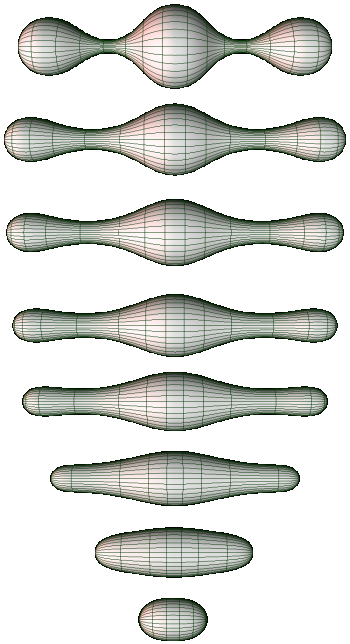
\includegraphics[width=13cm]{ricci-flow.png}
    %     \caption{Ricci flow visualization (Rubinstein, 2005)}
    %     % \label{fig:my_label}
    % \end{figure}

    
    
    
% \section{Exploratory }
    % Recent research in ML, Neuroscience, and Physics strengthens this direction of research; including the GLOM system for representing part-whole hierarchies in neural networks (Hinton 2021), similar part-whole investigations of biological neural trajectories using geometric analysis (Russo et al, 2020), as well as demonstrations of soliton generation from Bose-Einstein condensate. Examining pure mathematics research in ergodic theory and hyperbolic dynamics on moduli spaces enforces the ergodic free-energy minimizing model described in previous notebooks. An encoding mechanism using the cobordism property of the Yang-mills moduli space is also considered.
    
    
    % \subsection{Part-Whole Hierarchies}
    % In Artificial Neural Networks (Hinton 2021): \url{https://arxiv.org/abs/2102.12627}.
    
    % In the brain, using geometric analysis (Russo et al, 2020):
    
    % \url{https://www.sciencedirect.com/science/article/abs/pii/S0896627320303664}.
    
    % \url{https://www.sciencedirect.com/science/article/abs/pii/S0092867420312289}
    
    % \subsection{Cobordism}
    % Moduli of Yang–Mills connections have been most studied when the dimension of the base manifold $X$ is four. Here the Yang–Mills equations admit a simplification from a second-order PDE to a first-order PDE, the anti-self-duality equations. 
    % Additionally, these manifolds demonstrate a cobordism property where in specific circumstances (when the intersection form is definite) the moduli space of ASD instantons on a smooth, compact, oriented, simply-connected four-manifold $X$ gives a cobordism between a copy of the manifold itself, and a disjoint union of copies of the complex projective plane ${\displaystyle \mathbb {CP} ^{2}}$. This might provide a natural and gauge invariant method of dimensionality reduction to be applied to the hierarchical encoding and decoding of an upper bounding layer.
        

% \newpage
\textit{Work in progress}

% \subsubsection{Self-Organized Criticality}
%     Condensation of instantons (and noise-induced anti-instantons) are believed to be the explanation of the noise-induced chaotic phase known as self-organized criticality.

%     \url{https://arxiv.org/pdf/1102.1791.pdf}
    
%     parameterizing SOC by gaussian noise may be useful in drawing statistical comparisons between biological neural networks (via connectome harmonic analysis and the Abelian sandpile group) and quantum phenomena.

\begin{comment}
\section{Exploratory }
    \subsection{Cobordism}
        Moduli of Yang–Mills connections have been most studied when the dimension of the base manifold $X$ is four. Here the Yang–Mills equations admit a simplification from a second-order PDE to a first-order PDE, the anti-self-duality equations. 
        Additionally, these manifolds demonstrate a cobordism property where in specific circumstances (when the intersection form is definite) the moduli space of ASD instantons on a smooth, compact, oriented, simply-connected four-manifold $X$ gives a cobordism between a copy of the manifold itself, and a disjoint union of copies of the complex projective plane ${\displaystyle \mathbb {CP} ^{2}}$. This might provide a natural and gauge invariant method of dimensionality reduction to be applied to the hierarchical encoding and decoding of an upper bounding layer.
        
    \subsection{Part-whole Hierarchies}
    \subsubsection{In Artificial Neural Networks (GLOM)}
    
    \url{https://arxiv.org/abs/2102.12627}
    
    \subsubsection{In the Brain}
    \url{https://www.simonsfoundation.org/2021/04/07/geometrical-thinking-offers-a-window-into-computation/}
    
    \url{https://www.sciencedirect.com/science/article/abs/pii/S0092867420312289}
    
    \url{https://www.sciencedirect.com/science/article/abs/pii/S0896627320303664}
    
    
% \section{Ideas and Experiments}
%     does cobordism of moduli enable encoding via dimensionality reduction heirarchy. Symmetry/Guage equivarient hierarchical auto encoder. Symmetry of time to symmetry of space in particle and boson, next is approximate/broken symmetry in hierarchy (and lateral).  
    
%     If the brain indeed has ergodic dynamics imitable through a bernoulli scheme, then this architecture and 

%     The Abelian sandpile group describes a manifold that is able to be parameterized by its points of self-localized criticality.   The sandpile model is a rudimentary cellular automaton defined on a rectangular domain of the standard square lattice

%     Conversely, the computation of n a (lattice) gauge theory with unknown parameters can be done using machine learning techniques

    % on which inference can be performed using natural gradient descent where minima are
% \section{}
%     % https://arxiv.org/pdf/1705.05582.pdf
%     Machine Learning of Explicit Order Parameters: From the Ising Model to SU(2) Lattice Gauge Theory

% \subsection{Harmonic Model Interpretation}

% \subsubsection*{Connectome-Specific Harmonics}

% \subsubsection*{Abelian Sandpile Self-Local Criticality}
%     % https://www.pnas.org/content/116/8/2821
    
%     The Abelian sandpile model offers an interesting experimental opportunity for a manifold to be parameterized by its self-localized criticality. 
    
%     The sandpile model is a cellular automaton defined on a rectangular domain of the standard square lattice




% \subsection{Dimensionality Reduction}
% \subsubsection*{Cobordism}

\subsection{Dynamics}

\subsubsection{Ergodic theory on Moduli Spaces}

\url{https://annals.math.princeton.edu/articles/13160}

 Hyperbolic Dynamics

\url{http://scholarpedia.org/article/Hyperbolic_dynamics#Uniform_hyperbolicity}


\subsubsection{Connectome-specific Harmonic Waves}

\url{https://www.pnas.org/content/116/8/2821}

% See: The Hyperbolic Geometry of DMT Experiences

\subsubsection{Harmonic Dynamics of the Abelian Sandpile}
\url{https://www.pnas.org/content/116/8/2821}

%     Through the process of unfolding, i.e., passing from a polygonal billiard table to a Riemann manifold equipped with a holomorphic 1-form, a billiard trajectory which reflects off the sides of the table unfolds into a straight line or geodesic on the manifold. We define the symmetry group$ SL(X, \omega)$ associated to any translation surface. We extend the notions of ergodically optimal and topologically optimal to general translation surfaces. Finally, we introduce the notion of a lattice surface and compare it to an ergodically optimal surface.

\subsection{Physics}
    \subsubsection{Condesate of Instantons as Variational EBM}
    
    Energies can be thought of as being \textit{unnormalized negative log probabilities}. That is, we may use the Gibbs-Boltzmann distribution to convert an energy function to its equivalent probabilistic representation after normalization, i.e. $P(y \mid x)$. Recall, \textit{marginalisation} is a method that sums over the possible values of one variable to determine the marginal contribution of another. $P(y \mid x)$ is just an application of the Gibbs-Boltzmann formula with latent variables $z$ being marginalized implicitly through integration, i.e. $P(y \mid x) = \int_z P(y,z | x)$. Then,
    \begin{align*}
        P(y \mid x) &= \frac{ \int_z \exp(-\beta E(x,y,z)) }{ \int_y \int_z \exp(-\beta E(x, y, z))} \\
        % &= \frac{
        %     \exp \bigg [  -\beta (-\frac{1}{\beta} \log  \int_z \exp(-\beta E(x,y,z)) ) \bigg ]
        % }{
        %     \int_y \exp \bigg [  -\beta (-\frac{1}{\beta} \log  \int_z \exp(-\beta E(x,y,z)) ) \bigg ]
        % }
    \end{align*}
    The derivation introduces a $\beta$ term which is the inverse of temperature $T$, so as $\beta \rightarrow \infty$ the temperature goes to zero. $\beta$ is a positive constant that needs to be calibrated to fit the model. A larger $\beta$ value produces a more fluctuate model while a smaller $\beta$ gives a smoother model. When $\beta \rightarrow \infty$, we see that $\check{y} = \text{argmin}_{y} E(x,y)$. So we can redefine our energy function as an equivalent function using $F_\beta$,
    \begin{align*}
        F_{\infty} (x,y) &= \text{argmin}_z E(x,y,z)\\
        F_{\beta} (x,y) &= -\frac{1}{\beta} \log \int_z \exp(-\beta E(x,y,z)).
    \end{align*}
    
    In physics, $F_\beta$ is known as the free energy and $E$ is the energy. If we have a latent variable model and want to eliminate the latent variable $z$ in a probabilistically correct way, we just need to redefine the energy function in terms of $F_\beta$,
    \[
        P(y \mid x) = \frac{ \exp(-\beta F_\beta(x,y,z)) }{ \int_y \exp(-\beta F_\beta(x, y, z))}. \\
    \]
    
    \subsubsection{Self-Organized Criticality}
    In physics, instantons are particularly important because the condensation of instantons (and noise-induced anti-instantons) is believed to be the explanation of the noise-induced chaotic phase known as self-organized criticality.

    \subsubsection{Bose-Einstein Condesate and Solitons}
    
    Observation of Magnetic Solitons in a Bose-Einstein Condensate
    \url{https://physics.aps.org/articles/v13/s90}
    
    % https://www.researchgate.net/publication/51360828_Generating_Solitons_by_Phase_Engineering_of_a_Bose-Einstein_Condensate
    
    
    Spatial phase distributions were optically imprinted onto a Bose-Einstein condensate (BEC) of atoms and was shown to create solitons.
    
    \url{https://science.sciencemag.org/content/287/5450/97}
    
    \begin{multicols}{2}
    \noindent
    \begin{align*}
        {\displaystyle \,T_{\rm {c}}} \,  &\text{is the critical temperature,}\\
        \displaystyle \,n \, 	 &\text{ the particle density,}\\
        {\displaystyle \,m}	\, &\text{the mass per boson,}\\
        {\displaystyle \hbar } \, 	&\text{the reduced Planck constant,}\\
        {\displaystyle \,k_{\rm {B}}}\, 	&\text{the Boltzmann constant and}\\
        {\displaystyle \,\zeta }\, 	&\text{the Riemann zeta function;}
    \end{align*}
    \begin{align*}
        {\displaystyle T_{\rm {c}}=\left({\frac {n}{\zeta (3/2)}}\right)^{2/3}{\frac {2\pi \hbar ^{2}}{mk_{\rm {B}}}}}
    \end{align*}
    \end{multicols}
    \subsubsection*{Superliminal Solitons from Hyperbolic Shift Vectors}
    \url{https://arxiv.org/abs/2006.07125}




% \subsection*{Hyperbolic Dynamics}

% \subsubsection{Conformal Invariance}

    \subsection{Geometric Unity and Anthropic Principle}
    
    \url{https://geometricunity.nyc3.digitaloceanspaces.com/Geometric_Unity-Draft-April-1st-2021.pdf}
    
\end{comment} 

\section*{References}

\small

[1] Gao, Tingran. "The diffusion geometry of fibre bundles: Horizontal diffusion maps." Applied and Computational Harmonic Analysis 50 (2021): 147-215.
% https://arxiv.org/pdf/1602.02330.pdf

[2] Eckhard Meinrenken, "Principal bundles and connections", Lecture Notes. 
% http://www.math.toronto.edu/mein/teaching/moduli.pdf

[3] Tao, T. "What is a gauge?" (2008) https://terrytao.wordpress.com/2008/09/27/what-is-a-gauge/
% https://terrytao.wordpress.com/2008/09/27/what-is-a-gauge/

[4] Wetzel, Sebastian J., and Manuel Scherzer. "Machine learning of explicit order parameters: From the Ising model to SU (2) lattice gauge theory." Physical Review B 96.18 (2017): 184410.
% https://arxiv.org/pdf/1705.05582.pdf


[5] Du, Yilun, and Igor Mordatch. "Implicit generation and generalization in energy-based models." arXiv preprint arXiv:1903.08689 (2019).
% https://arxiv.org/abs/1903.08689

[6] Blei, David M., Alp Kucukelbir, and Jon D. McAuliffe. "Variational inference: A review for statisticians." Journal of the American statistical Association 112.518 (2017): 859-877.

% [3] Paul, Arnab, and Suresh Venkatasubramanian. "Why does deep learning work?-a perspective from group theory." arXiv preprint arXiv:1412.6621 (2014).
% https://arxiv.org/pdf/1412.6621.pdf

[7] Hinton, Geoffrey. "How to represent part-whole hierarchies in a neural network." arXiv preprint arXiv:2102.12627 (2021).

[8] Hinton, Geoffrey E. "Mapping part-whole hierarchies into connectionist networks." Artificial Intelligence 46.1-2 (1990): 47-75.

[9]  Yann LeCun  and Alfredo Canziani. "DEEP LEARNING". DS-GA 1008, SPRING 2020. NYU CENTER FOR DATA SCIENCE

[10] Russo, Abigail A., et al. "Neural trajectories in the supplementary motor area and motor cortex exhibit distinct geometries, compatible with different classes of computation." Neuron 107.4 (2020): 745-758.

[11] Farolfi, A., et al. "Observation of magnetic solitons in two-component Bose-Einstein condensates." Physical Review Letters 125.3 (2020): 030401.

[12] Denschlag, J., et al. "Generating solitons by phase engineering of a Bose-Einstein condensate." Science 287.5450 (2000): 97-101.

[13] J. Hyam Rubinstein and Robert Sinclair. "Visualizing Ricci Flow of Manifolds of Revolution", Experimental Mathematics v. 14 n. 3, pp. 257–384

[14] Jaini, Priyank, Lars Holdijk, and Max Welling. "Learning Equivariant Energy Based Models with Equivariant Stein Variational Gradient Descent." arXiv preprint arXiv:2106.07832 (2021).

[15] I.V. Ovchinnikov. Self-organized criticality as Witten-type topological field theory with spontaneously
broken Becchi-Rouet-Stora-Tyutin symmetry. Physical Review E, 83,051129 (2011).

[16] Zhai, Jian, Chaojun Yu, and You Zhai. "Witten-type topological field theory of self-organized criticality for stochastic neural networks." arXiv preprint arXiv:2106.10851 (2021).

[17] Michael Jablonski and Andrea Young,Ricci Yang-Mills solitons on nilpotent Lie groups, J. Lie Theory23(2013),no. 1, 177–202. MR 3060772

% https://ncatlab.org/nlab/show/principal+bundle


% % % % % % % % % % % % % % % % % % % % % % % % % % % % % % % % % % % % 






\end{document}
